\documentclass[12pt]{article}

\usepackage{amsmath}
\usepackage{mathtools}
\DeclarePairedDelimiter\ceil{\lceil}{\rceil}

\usepackage{algorithm}

\usepackage{algorithmic}

\usepackage{enumitem}

\usepackage{amssymb}

\usepackage{graphicx}

\usepackage{hyperref}

\usepackage[utf8]{inputenc}

\title{Les méthodes exactes}

\begin{document}
\maketitle

Dans ce chapitre,nous allons présenter la conception détaillée des méthodes exactes sur lesquelles notre choix d'implementation s'est porté:

\begin{enumerate}

\item Le branch and bound

\item Une version améliorée du branch and bound

\item La recherche exhaustive

\item La programmation dynamique
\end{enumerate}
Dans le but de montrer l’applicabilité de ces méthodes, comparer leurs performances et montrer leurs limites, nous effectuerons des tests empiriques et comparatifs sur des benchmarks d’un coté, et sur des instances générées par notre propre générateur d’instances d’un autre coté.
\section{Branch and bound}
\begin{itemize}
    \item L'algorithme Branch-and-Bound (B \&B) que nous avons implémenté tente de ranger un objet à la fois en fonction de l’ordre initial des objets. 
    \item Au niveau j de l’arbre, B \&B crée un noeuds fils pour chaque boite ouverte et range l’objet j dans cette boîte si c’est possible. il crée aussi un noeuds supplémentaire qui représente l’ouverture d’une nouvelle boîte, et il range l’objet j dans cette boîte.
    \item En pratique, au niveau 1 de l’arbre l’objet 1 est rangé dans la boîte 1 , au niveau 2 l’objet 2 est rangé dans la boîte 1 ou dans une nouvelle boîte 2 ,...etc 
    \item A chaque noeud, on résout un sous problème de taille (n-k) du bin packing, où les k premiers objets ont déjà été emballés.
    \item L’opération du rangement d’un objet i au niveau k consiste à permuter entre les éléments list(K) et list(i). On va avoir comme sortie une liste d’objets ordonnées selon l’ordre de rangement, il suffit ensuite de remplir les boîtes par les objets dans leur nouvel ordre pour générer la solution (l’emplacement de chaque objet dans les boîtes) 
\end{itemize}

\begin{figure}[h]
    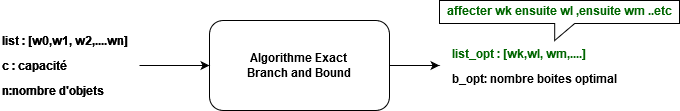
\includegraphics[width=\linewidth]{../figures/diagr1.png}
\end{figure}
\subsection{Pseudo-Code}
Soient:
\begin{itemize}
    \item n : le nombre d’articles 
    \item list[0… n-1] : la liste des articles en entrées 
    \item opt\_list: la list ordonnée fournissant la solution optimale en sortie 
    \item opt\_cost: le nombre de boîtes optimal
    \item C:la capacité maximale d’une boîte. 
\end{itemize}

L’algorithme proposé est une fonction récursive packBins ayant comme paramètres:
\begin{itemize}
    \item k:l’ordre de l’élément à être ranger ( le niveau dans l’arbre).
    \item sumwt:la somme des poids des éléments restants à être rangés
    \item bcount:la somme cumulée des boîtes déjà utilisées ( depuis la racine jusqu’à ce nœud)
    \item capa\_restante:l’espace libre restant dans la boîte ouverte.
     
\end{itemize}

\begin{algorithm}[H]
    \caption{Branch \& Bound}
    \begin{algorithmic}
    \IF{$n=k$}
        \STATE //noeud feuille (n objets rangés)
        \IF{$bcount<opt\_cost$}
            \STATE //solution exacte obtenue par cette branche est meilleure que celle trouvée auparavant
            \STATE màj du coût optimal $opt\_cost=bcount$ .
            \STATE sauvegarder la solution liste  $opt\_list=liste$. 
        
        \ELSE
            \STATE continuer le parcours,parcours (monter d’un niveau dans l’arbre).
       \ENDIF
        
    \ELSE

        \STATE //L’ensemble des articles restants sont dans les positions list[k… n-1].
        \STATE //chaque nœud fils i signifie qu’on a rangé le ième article parmi les articles restants (ayant la position k+i dans la liste list) à la position k.
        \FOR{ chaque nœud fils i }
            \STATE Mettre l’article list[k+i] dans une boîte en permutant l’article[k+i] avec l’article[k] : permuter(k+i,k) .
            \STATE Incrémenter le nombre de boîtes utilisées (bcount) si on a ouvert une nouvelle boite.
            \STATE Mettre à jour la capacité restante (capa\_restante).
            \STATE Mettre à jour la somme des volume des articles restants à être ranger (Sumwt)
            \STATE Calculer l’évaluation du nœud fils courant (borne L1) : $Bound=bcount+\frac{(sumwt-capa\_restante)}{C}$
            \STATE Comparer l’évaluation du nœud avec la solution optimale courante :
            \IF{$bcount\geq opt\_cost$}
                \STATE //solution exacte obtenue par cette branche est meilleure que celle trouvée auparavant
                \STATE  le nœud est éliminé. Dans ce cas on re-permute pour revenir à l’état précédant (permute (k+i,k)). 
                \STATE sauvegarder la solution liste  $opt\_list=liste$ 
        
           \ELSE
                \STATE on exploite le nœud courant encore, en faisant un appel récursif à la fonction avec la valeur  k+1 dans le 1 paramètre,en utilisant les nouvelles valeurs des autres paramètres.
           \ENDIF


        \ENDFOR
    \ENDIF
    \end{algorithmic}
    \end{algorithm}
\subsubsection*{Evaluation d'un noeud (Borne L1)}
L’évaluation d’un nœud est calculée en sommant 2 parties, le nombre de boîtes déjà utilisées bcount et une estimation du nombre de boîtes qu’on va ouvrir encore pour contenir les objets restants. Cette estimation est obtenue en divisant la somme des poids restants sumwt sur la capacité d’une boîte. On soustrait de la somme des poids restants, l’espace vide 
restant dans la dernière boîte ouverte, car ce dernier peut contenir des objets. On obtient ainsi la formule suivante :  

\begin{figure}[h!]
    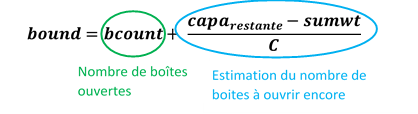
\includegraphics[width=8cm]{../figures/formule1.png}
\end{figure}
\paragraph{exemple 1: }
List= {10,50,25,80,70,75,35,70} ;   C = 100 
\begin{figure}[h!]
    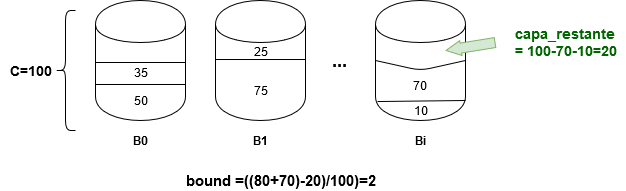
\includegraphics[width=10cm]{../figures/example1.png}
\end{figure}
\paragraph{exemple 2: }
n= 5 ; $W_{j}$={49,41,34,33,29} ; c=100 
on pose : $b_j$= le numéro de boîte qui contient l’objet j.

\begin{figure}[h!]
    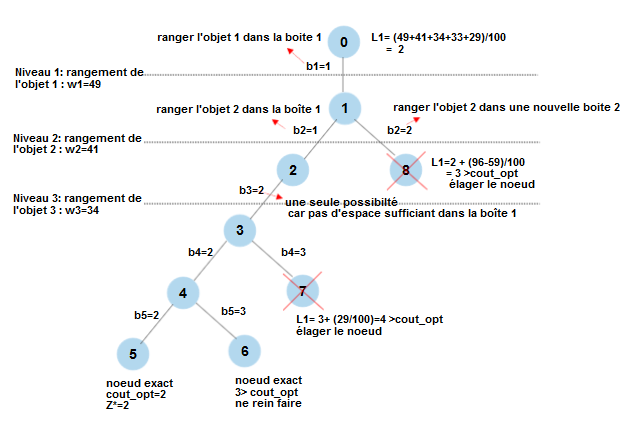
\includegraphics[width=\linewidth]{../figures/diag2.png}
\end{figure}
\section{Branch and bound amélioré}
Une version améliorée de l’algorithme Branch and Bound présenté ci-dessus. L’amélioration s’est faite en 2 étapes: 
\begin{enumerate}
    \item Utilisation de l’heuristique WFD (Worst Fit Decreasing) pour initialiser la solution optimale.
    \item Changement de la borne L1 utilisée par une autre borne plus puissante appelée L2. 
\end{enumerate}
\subsection*{Evaluation d'un noeud (Borne L2)}
Il a été prouvé que la borne L1 n’est efficace que quand les poids des objets sont petits, c’est à dire qu’on peut mettre plusieurs objets dans la même boîte. Si ce n’est pas le cas, et que les objets ont de grands poids ( proches de C) , cette borne n’aura aucun effet et l’algorithme fera une recherche exhaustive. 
C’est pour cela que la borne L2 à été proposée par Martello et Toth ,pour remédier à ce problème. 
on rappelle la formule de la borne L2, qui a été déjà présentée dans l’état de l’art:
\paragraph{rappel}
Soit \(\alpha\) un entier tels que :
\[0 \le \alpha \le C/2\]
On definie des classes d'articles suivantes: 
\[C_1 = \{a_i, \quad C-\alpha < v_i\} \]
\[C_2 = \{a_i, \quad C/2 < v_i \le C-\alpha\} \]
\[C_3 = \{a_i, \quad \alpha < v_i \le C/2\} \]
\(BI(I)\)  est donnée par la formule suivante:
\[BI(I)=max\{L(\alpha),\quad 0 \le \alpha \le C/2\}\]
Avec
\[L(\alpha)=|C_1|+|C_2|+max(0, \ceil*{\frac{\sum_{j \in C_3}^{} v_j - (|C_2|*C - \sum_{j \in C_2}^{} v_j) }{C}})\]
\paragraph{Explication de la formule :}
Etant donnée que les objets des classes $C_1$ et $C_2$ ont un poids supérieur à $C/2$ chacun d'eux sera placé dans une boîte séparée pour le contenir, donc
$|C_1|+|C_2|$boîtes sont utilisées quelque soit la solution. De plus,aucun objet de l’ensemble $C_3$ ne peut être rangé dans une boîte contenant un objet de $C_1$ ( à cause de la contrainte de capacité). La capacité résiduelle (espace libre) des
$|C_2|$ boîtes est de : $C^*=|C_2|*c-\sum_{j \in C_2}^{} w_j$
Donc dans le meilleur des cas, cette capacité résiduelle va être remplie par les objets de $C_3$, et dans ce cas le nombre de nouvelles boîtes qu’on doit ouvrir est de :  
$\frac{\sum_{j \in C_3 -C^*}^{} w_j}{c}$ ( cette dernière formule utilise le même principe que la borne L1).
\subsection{Pseudo-Code}
\begin{algorithm}[H]
   \caption{Branch and bound amélioré }
   \begin{algorithmic} 
   \STATE Appliquer WFD sur l’instance pour initialiser le coût optimal:\linebreak cout\_opt=WFD(problème)
   \STATE Appliquer l’algorithme Branch and Bound sur le problème en utilisant la borne L2
   \end{algorithmic} 
\end{algorithm}
\section{Recherche exhaustive }
Dans cette 3ème solution, on a implémenté une recherche exhaustive, qui consiste à parcourir l’ensemble des nœuds et leurs fils, sans aucun élagage de nœuds. Donc on aura le même algorithme que celui du branch and bound, en supprimant l’étape de l’évaluation du nœud pour décider de son élagage.  
\section{La programmation dynamique }
\paragraph{principe }
Étant donnée une liste L de N articles à ranger et la capacité d’une boîte C :
\subparagraph{\underline{structure de donnée :}}
\begin{itemize}
    \item La table de vérité m : une matrice de (C+1) colonnes, et N lignes, tel que m[i][j] désigne si l’article i peut être rangé dans une capacité j.
\end{itemize}
\subparagraph{\underline{Etapes :}}
\begin{enumerate}
    \item Remplir la table de vérité correspondante au problème actuel (L,C), puis ouvrir une nouvelle boite
    \item En parcourant la table de vérité, choisir les articles à mettre dans cette nouvelle boite.
    \item Ranger les articles choisis dans la boîte, et mettre à jour la liste L (retirer ces articles de L). 
    \item Réitérer le processus jusqu’à avoir rangé tous les articles (N=0) 
\end{enumerate}
\subsection{Pseudo-Code}
\subsubsection{Méthodes utilisées :}
\paragraph{la méthode : get\_truth\_table(capacité, items):}
\subparagraph{paramètres:}
\begin{itemize}
    \item capacité : la capacité d’une boîte
    \item items : la liste des articles de poids $W_j$ à ranger
\end{itemize}
\subparagraph{Rôle :}
Création et initialisation de la table de vérité
\begin{algorithm}[H]
    \caption{get\_truth\_table(capacité, items)}
    \begin{algorithmic} 
    \STATE Initialiser toutes les cases de la table de vérité m à “true” 
    \STATE Parcourir les articles un à un //les lignes de la matrice m
    \FOR{chaque article i }
        \FOR{chaque colonne j } 
            \STATE ///parcourir la capacité une unité par une unité
            \IF{$i=0$}
                \STATE //premier article
                \IF{$j>0 et j \ne W_j$}
                    \STATE //c’est à dire cette capacité ne pourra pas accueillir l’article courant
                    \STATE Mettre "faux" dans la case
                    \STATE //revient à remplir la première ligne par “false”, sauf la case1 et la case qui correspond au volume de l’article
                
                
                    
                    
                \ENDIF
                
          \ELSE

                \STATE //pour le reste des articles, utiliser la relation suivante sur la table
                \IF{$ j<W_j$}
                    \STATE m[i][j] = m[i-1][j] //la valeur de la case en dessus
                \ELSE
                    \STATE  $m[i][j] = m[i-1][j] \vee m[i-1][j-(W_i)]$


                \ENDIF
          \ENDIF
        \ENDFOR
    \ENDFOR
    \RETURN m
    \end{algorithmic} 
 \end{algorithm}
 \paragraph{la méthode : get\_truth\_table(capacité, items):}
\subparagraph{paramètres:}
\begin{itemize}
    \item m : table de vérité
\end{itemize}
\subparagraph{Rôle :}
Choisir les articles à mettre dans la boîte 
\begin{algorithm}[H]
    \caption{get\_truth\_table(capacité, items)}
    \begin{algorithmic} 
    \STATE K = (nombre de lignes de m) - 1 // indice de la dernière ligne
    \STATE Initialiser la liste des indices des articles choisis à la liste vide : picked\_items\_indices = []
    \IF{$k\geq 0$}
        \STATE $k = max( j tel que m[k][j]=true)$ //prendre la plus grande capacité totale
          
    \ENDIF
    \WHILE{$k\geq 0$}
        \STATE //tant qu’il nous reste encore de lignes à visite
            \IF{$k=0 et j>0 $}
                \STATE //première ligne
                \STATE ajouter l’article k à picked\_items\_indices
               
            \ELSE
                \IF{$ m[k-1][j] = false$}
                    \STATE ajouter l’article k à picked\_items\_indices
                    \STATE j = j - $W_k$

                \ENDIF
            \ENDIF
            \STATE  $k = k-1$ //allez à la ligne de dessus      
   \ENDWHILE
    \RETURN picked\_items\_indices
    \end{algorithmic} 
 \end{algorithm}
 \paragraph{la méthode : \_move\_items\_to\_bin(list\_of\_items\_indices, bin\_index)}
 \subparagraph{paramètres:}
 \begin{itemize}
     \item list\_of\_items\_indices : liste des indices des articles de poids $W_j$
     \item bin\_index : le numéro de la boîte de destination
 \end{itemize}
 \subparagraph{Rôle :}
 Ranger les articles dans la boîte 
 \begin{algorithm}[h!]
     \caption{ \_move\_items\_to\_bin(list\_of\_items\_indices, bin\_index)}
     \begin{algorithmic} 
        \FOR{chaque article à indice dans list\_of\_items\_indices  }
            \STATE Ranger l’article dans la boîte ayant l’indice bin\_index
        \ENDFOR
    
    \end{algorithmic} 
  \end{algorithm}
\subsubsection{Méthode principale :}
\paragraph{La méthode: Pack\_items()}
  \subparagraph{Rôle :}
  ranger les articles dans un nombre min de boîte , en retournant la solution optimale et son coût ( nombre de boîtes utilisées)
 \begin{algorithm}[H]
     \caption{ \_move\_items\_to\_bin(list\_of\_items\_indices, bin\_index)}
     \begin{algorithmic} 
       \WHILE{il reste encore des articles à ranger dans la liste L }
            \STATE Construire la table de vérité m : m=get\_truth\_table(capacité, items)
            \STATE  bin\_index = Ouvrir une nouvelle boîte
            \STATE  Ajouter la nouvelle boîte à la liste des boîtes
            \STATE   picked\_items = \_pick\_items(m) // choix des avrticles à ranger dans la boîte i 
            \STATE  \_move\_items\_to\_bin(picked\_items, bin\_index) // ranger les articles dans la boîte i
            \STATE   Mettre à jour la liste L, en retirant les articles rangés


        \ENDWHILE
    \end{algorithmic} 
  \end{algorithm}
  \subsubsection*{Exemple :}
  Capacité=5;Articles={1,5,2}
  \paragraph{première itération :}
  Construction de la table de vérité:\linebreak
  \begin{figure}[h!]
    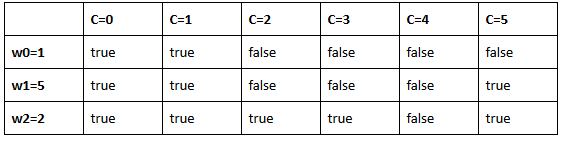
\includegraphics[width=10cm]{../figures/tabit1.png}
\end{figure}
\begin{itemize}
    \item Ouvrir une nouvelle boîte $B_0$ avec une capacité = 5
    \item Choisir les articles à mettre dedans : il choisit l’article $W_1$=5 
    \item Mettre l’article $W_1$ choisi dans la boîte $B_0$
    \item Enlever l’article rangé de la liste des articles à ranger.


\end{itemize}
\paragraph{deuxième itération :}
Construction de la table de vérité:\linebreak
\begin{figure}[H]
  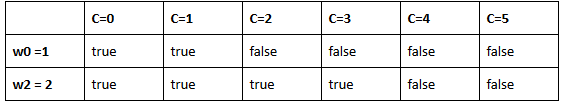
\includegraphics[width=10cm]{../figures/tabit2.png}
\end{figure}
\begin{itemize}
  \item Ouvrir une nouvelle boîte $B_1$ avec une capacité = 5
  \item Choisir les articles à mettre dedans : il choisit l’article $W_0$=1 et l’article $W_2$=2
  \item Mettre les articles $W_0$ et $W_2$ choisis dans la boîte $B_1$
  \item Enlever les articles rangés de la liste des articles à ranger. 
\end{itemize}
\paragraph{troisième itération :}
\begin{itemize}
    \item Liste vide
\end{itemize}
ARRÊT DE L’ALGORITHME
\paragraph{La solution optimale:}
\begin{itemize}
    \item $B_0$ contiendra l'article $W_1$ avec un taux d'occupation=$5/5 =100\%$
    \item $B_1$ contiendra les articles $W_0$ et $W_2$ avec un taux d'occupation=$ (1+2)/5 =  60\%$
  \end{itemize}

\end{document}